\documentclass[11pt,a4paper]{article}
\usepackage[margin=1in]{geometry}
\usepackage[T1]{fontenc}
\usepackage{lmodern}
\usepackage{microtype}
\usepackage{amsmath,amssymb,amsthm}
\usepackage{mathtools}
\usepackage{booktabs}
\usepackage{enumitem}
\usepackage{xcolor}
\usepackage[hidelinks]{hyperref}
\usepackage{tikz}
\usetikzlibrary{arrows.meta,positioning,calc}

\newtheorem{theorem}{Theorem}[section]
\newtheorem{proposition}[theorem]{Proposition}
\newtheorem{lemma}[theorem]{Lemma}
\newtheorem{corollary}[theorem]{Corollary}
\newtheorem{hypothesis}[theorem]{Hypothesis}
\theoremstyle{definition}
\newtheorem{definition}[theorem]{Definition}
\newtheorem{remark}[theorem]{Remark}
\newtheorem{prediction}[theorem]{Prediction}

\newcommand{\phig}{\varphi}
\newcommand{\Jcost}{J}
\newcommand{\Rhat}{\hat{R}}
\newcommand{\Zp}{Z}
\newcommand{\code}[1]{\texttt{\small #1}}
\newcommand{\forced}[1]{\noindent\textbf{Status: Forced.} #1}
\newcommand{\bridge}[1]{\noindent\textbf{Status: Bridge hypothesis.} #1}
\emergencystretch=1em

\title{\textbf{Four Channel Groups from One Cost}\\[0.5em]
\large A Machine-Verified Decomposition of the Recognition Science\\
Death Projection}
\author{Jonathan Washburn\\
\small Recognition Science Research Institute, Austin, Texas\\
\small \texttt{washburn.jonathan@gmail.com}}
\date{March 2026}

\begin{document}
\maketitle

\begin{abstract}
The Recognition Composition Law (RCL) forces an 8-channel octave
structure whose death projection decomposes into exactly four groups
with multiplicities $(3,1,3,1)$. Two structural features are forced:
the octave midpoint partitions channels into low-frequency
($<4$) and persistent ($\ge 4$) halves, and the maximum-index slot
uniquely maximizes the preservation budget. Two bridge hypotheses
complete the decomposition: (H1) the transition boundary sits at the
midpoint minus one, giving a $3{+}1{+}4$ split; (H2) the transitional
gate opens at the first reflexivity level where cost exceeds kernel
dimension, forcing $k{=}3$. Under H1--H2, the resulting four groups
have distinct survival laws and support a unique rank-preserving
bijection to any ordered four-level external taxonomy. All results are
formalized in Lean~4 with zero \texttt{sorry} obligations. Every claim
is labeled as forced, bridge, or interpretive.
\end{abstract}

\tableofcontents

%% =====================================================================
\section{Introduction}
\label{sec:intro}
%% =====================================================================

This paper studies the internal structure of the Recognition Science
(RS) death projection. The central question is:
\emph{what forced decomposition does the 8-channel octave admit when an
embodied recognition boundary dissolves?}

The answer is partly forced and partly bridged. The RS core already
determines an 8-channel octave, a monotone preservation budget
$B(k)=\phig^k$, and a unique maximum-budget slot. Two additional bridge
hypotheses complete a four-group decomposition with multiplicities
$(3,1,3,1)$.

To maintain rigorous provenance, every claim carries one of three
labels:
\begin{itemize}
\item \textbf{Forced}: derived from the RS core (T0--T8) and
  machine-verified in Lean~4.
\item \textbf{Bridge hypothesis}: a principled structural claim
  not yet derived from the RS core.
\item \textbf{Interpretive}: a semantic identification connecting
  the formal structure to external language.
\end{itemize}

\subsection{Scope}

This is a mathematical investigation within the RS axiom system.
It derives what the axioms force under stated hypotheses. It is not an
empirical paper and does not attempt to establish any historical,
phenomenological, or theological claim. The derivation is
machine-verified in Lean~4 with zero \texttt{sorry} obligations.

%% =====================================================================
\section{Related Work}
\label{sec:related}
%% =====================================================================

Several mathematical frameworks model aspects of consciousness.
Tononi's Integrated Information Theory
(IIT)~\cite{Tononi2004,Oizumi2014} assigns an integration scalar to a
system, Penrose's work~\cite{Penrose1994} links consciousness to
foundational physics, and Hoffman's conscious realism~\cite{Hoffman2019}
treats conscious agents as primitive. None of these derive a discrete
four-group decomposition of a death transition from a single
functional equation. In that sense, the present paper is not a survey
of consciousness models but a provenance analysis of one specific RS
claim.

%% =====================================================================
\section{The RS Forcing Chain}
\label{sec:forcing}
%% =====================================================================

Recognition Science derives structure from the
\textbf{Recognition Composition Law} (RCL):
\begin{equation}
\label{eq:RCL}
\Jcost(xy) + \Jcost(x/y)
= 2\Jcost(x)\Jcost(y) + 2\Jcost(x) + 2\Jcost(y).
\end{equation}
With normalization $\Jcost(1)=0$ and calibration
$\Jcost''_{\ln}(0)=1$, the unique solution is~\cite{Washburn2026axioms}
\begin{equation}
\label{eq:Jcost}
\Jcost(x) = \tfrac{1}{2}(x + x^{-1}) - 1 = \cosh(\ln x) - 1.
\end{equation}

The complete forcing chain (T0--T8) derives, in order:
logic, the meta-principle, discreteness, ledger structure,
recognition events, the unique cost, the golden ratio,
the 8-tick period, and spatial dimension $D=3$.

For the present paper, the critical forced outputs are:
\begin{enumerate}[label=(\roman*)]
\item $\phig$ is the unique positive root of $x^2=x+1$.
  \hfill \forced{Lean: \code{phi\_sq\_eq}.}
\item The 8-tick period yields 8 abstract information channels.
  \hfill \forced{Lean: \code{octave\_slot\_count\_from\_t7}.}
\item The reflexivity eigenvalue satisfies $\lambda^2=\lambda+1$,
  hence $\lambda=\phig$.
  \hfill \forced{Lean: \code{reflexivityEigenvalue\_sq}.}
\item The capacity recursion
  $C(0)=1$, $C(k{+}1)=\phig\cdot C(k)$ gives
  $B(k)=\phig^k$.
  \hfill \forced{Lean: \code{informationCapacity\_eq\_pow}.}
\end{enumerate}

%% =====================================================================
\section{The Death Projection}
\label{sec:death}
%% =====================================================================

When an embodied recognition boundary dissolves, RS models the
transition as a diagonal projection
$\mathcal{D}: \mathcal{H}_{\mathrm{emb}} \to \mathcal{H}_{\mathrm{light}}$
on an 8-channel state.

Two facts are forced from the RS core:

\begin{theorem}[$\Zp$-Pattern Conservation]
\label{thm:z-conservation}
The identity invariant $\Zp$ is preserved through dissolution and
re-embodiment.

\forced{Lean: \code{dissolution\_certificate\_preserves\_Z},
\code{Z\_survives\_death}, \code{Z\_survives\_rebirth}.}
\end{theorem}

\begin{theorem}[Projection Monotonicity]
\label{thm:proj-mono}
For any admissible retention mask $0 \le m_j \le 1$,
$I_{\mathrm{proj}} \le I_{\mathrm{tot}}$.

\forced{Lean: \code{projectedInformation\_le\_total}.}
\end{theorem}

The unresolved question is the internal grouping of these channels
under dissolution.

%% =====================================================================
\section{Forced Structural Features}
\label{sec:forced}
%% =====================================================================

Two features of the 8-channel death projection are forced without
additional hypotheses.

\subsection{Octave Midpoint}

\begin{theorem}[Octave Midpoint]
\label{thm:midpoint}
The 8-tick octave has a structural midpoint
$N_{\mathrm{mid}} = \lfloor 8/2 \rfloor = 4$.
This divides the 8 channels into:
\begin{itemize}
\item a low-frequency half: slots $0,1,2,3$,
\item a persistent half: slots $4,5,6,7$.
\end{itemize}

\forced{Lean: \code{octaveMidpoint\_from\_eight\_tick}.}
\end{theorem}

The persistent half matches the proved condition
$\mathrm{isZStructural}(c) \iff \iota(c)\ge 4$
(Lean: \code{z\_structural\_iff\_above\_midpoint}).

\subsection{Maximum-Budget Slot}

\begin{theorem}[Budget Maximizer]
\label{thm:max-budget}
The preservation budget $B(k)=\phig^k$ is strictly monotone.
Among the 8 channels, slot~7 uniquely maximizes the budget:
\[
  B(\iota(c)) < B(7) \quad \forall c \ne \mathrm{reflexivity}.
\]

\forced{Lean: \code{reflexivity\_is\_max\_slot},
\code{z\_carrier\_at\_top}.}
\end{theorem}

This is purely structural: $\phig^k$ increases with $k$, and the slot
index never exceeds~7.

%% =====================================================================
\section{Bridge Hypotheses}
\label{sec:bridge}
%% =====================================================================

Two bridge hypotheses, not yet derived from the RS core, are needed to
complete the four-group decomposition.

\begin{hypothesis}[Transition Boundary at $N_{\mathrm{mid}}-1$]
\label{hyp:boundary}
The boundary between substrate-dependent and transitional channels
sits at $N_{\mathrm{mid}}-1 = 3$, not at $N_{\mathrm{mid}} = 4$.
That is:
\begin{align}
\mathrm{substrate\text{-}dependent}(c) &\iff \iota(c) < 3,\\
\mathrm{transitional}(c) &\iff \iota(c) = 3.
\end{align}

\bridge{A derivation would need to show that the DFT-8 conjugate
pairing gives slot~3 a distinguished transitional role. The current
formalization proves only consistency with the existing bridge
predicates.}
\end{hypothesis}

\begin{hypothesis}[Cost-Crossing Transitional Gate]
\label{hyp:gate}
The transitional channel activates at the first reflexivity level $k$
where $\phig^k - 1 \ge \dim(\ker\mathcal{D})$.

\bridge{The numerical consequence is clean, but the principle that the
gate criterion is cost-to-kernel crossing is not currently derived from
the RS axioms.}
\end{hypothesis}

\begin{theorem}[Threshold under H\ref{hyp:gate}]
\label{thm:threshold}
Under Hypothesis~\ref{hyp:gate}, the transitional threshold is $k^*=3$.
\end{theorem}

\begin{proof}
$\phig^2 - 1 = \phig < 3$ while $\phig^3 - 1 > 3$.
\forced{Lean: \code{emotional\_threshold\_forced\_at\_three}.}
\end{proof}

%% =====================================================================
\section{The Four-Group Decomposition}
\label{sec:four}
%% =====================================================================

Under Hypotheses~\ref{hyp:boundary} and~\ref{hyp:gate}, the 8 channels
decompose into four groups with distinct post-dissolution behavior.

\begin{theorem}[Four-Group Decomposition under H1--H2]
\label{thm:tetrachotomy}
The channel-group assignment is determined by the octave-slot index:
\[
  \mathrm{group}(c) =
  \begin{cases}
    \mathrm{Group}_0 & \iota(c) < 3,\\
    \mathrm{Group}_1 & \iota(c) = 3,\\
    \mathrm{Group}_3 & \iota(c) = 7,\\
    \mathrm{Group}_2 & 4 \le \iota(c) \le 6.
  \end{cases}
\]
The four groups have cardinalities $(3,1,3,1)$ summing to~8.

\forced{Conditional on H1--H2. Lean:
\code{channelToGroup\_forced\_by\_structure},
\code{four\_classes\_forced}.}
\end{theorem}

\begin{proof}
Hypothesis~\ref{hyp:boundary} separates slots $<3$ from slot~3.
Theorem~\ref{thm:max-budget} separates slot~7 from slots $4$--$6$.
The remaining multiplicities follow by enumeration.
\end{proof}

\begin{center}
\small
\begin{tabular}{llll}
\toprule
\textbf{Group} & \textbf{Channels} & \textbf{Survival law} & \textbf{Status} \\
\midrule
$\mathrm{Group}_0$ & 0--2 & zero survival & conditional on H1 \\
$\mathrm{Group}_1$ & 3 & threshold-gated survival & conditional on H1+H2 \\
$\mathrm{Group}_2$ & 4--6 & finite persistent budget & forced from midpoint split \\
$\mathrm{Group}_3$ & 7 & maximal budget, $\Zp$-carrier candidate & forced from max-budget \\
\bottomrule
\end{tabular}
\end{center}

\subsection{Maximum-Budget Identification}

We identify the conserved $\Zp$-pattern with the maximum-budget slot
(slot~7). This is a natural structural identification, motivated by the
principle that an indestructible invariant should occupy the most
persistent channel.

\bridge{Deriving the principle ``conserved topological invariants
maximize budget'' from the RS core remains an open problem.}

%% =====================================================================
\section{Ordered Four-Level Interfaces}
\label{sec:convergence}
%% =====================================================================

The four-group decomposition determines a generic interface theorem.

\begin{definition}[Dissolution Rank]
\label{def:rank}
Let $r: \mathrm{ChannelGroup} \to \mathrm{Fin}(4)$ be the injective
rank function
\[
  r(\mathrm{Group}_0)=0,\quad
  r(\mathrm{Group}_1)=1,\quad
  r(\mathrm{Group}_2)=2,\quad
  r(\mathrm{Group}_3)=3.
\]
\end{definition}

\begin{theorem}[Rank-Preserving Uniqueness]
\label{thm:unique-map}
Let $\alpha$ be any four-element set with a rank
$\rho: \alpha \to \mathrm{Fin}(4)$.
Any bijection $f: \alpha \to \mathrm{ChannelGroup}$ satisfying
$r(f(a)) = \rho(a)$ for all $a$ is unique.

\forced{Lean: \code{rank\_preserving\_map\_unique}.}
\end{theorem}

\begin{proof}
If $f$ and $g$ both preserve rank, then
$r(f(a))=\rho(a)=r(g(a))$ for each $a$.
Injectivity of $r$ implies $f(a)=g(a)$.
\end{proof}

\begin{corollary}[Universal Four-Level Interface]
\label{cor:forced-maps}
Any ordered four-level external taxonomy admits exactly one
rank-preserving bijection to the RS channel groups.
\end{corollary}

\begin{remark}
The current codebase contains several concrete four-level instantiations
of this interface theorem. The present paper suppresses their historical
or external naming and records only the generic structural result.
\end{remark}

%% =====================================================================
\section{Dissolution Timing}
\label{sec:timing}
%% =====================================================================

The $\phig$-ladder yields a strict hierarchy of persistence:

\begin{theorem}[Dissolution Hierarchy]
\label{thm:hierarchy}
\[
  r(\mathrm{Group}_0) < r(\mathrm{Group}_1) <
  r(\mathrm{Group}_2) < r(\mathrm{Group}_3).
\]

\forced{Lean: \code{dissolution\_strict\_hierarchy}.}
\end{theorem}

\subsection{Structural Ordering Predictions}

Without a calibrated base timescale, RS predicts only the ordering of
dissolution:
\begin{enumerate}
\item $\mathrm{Group}_0$ dissolves first.
\item $\mathrm{Group}_1$ dissolves next if activated.
\item $\mathrm{Group}_2$ persists longer with a finite budget.
\item $\mathrm{Group}_3$ is maximally persistent.
\end{enumerate}

\subsection{Budget Bounds}

The relative scale of persistence is governed by:
\begin{center}
\small
\begin{tabular}{lll}
\toprule
\textbf{Group} & \textbf{Budget} & \textbf{Numerical range} \\
\midrule
$\mathrm{Group}_0$ & $0$ & zero survival \\
$\mathrm{Group}_1$ & $\phig^3$ (conditional) & $4.0 < B < 4.25$ \\
$\mathrm{Group}_2$ & $[\phig^4,\phig^6]$ & $6.9 < B < 17.9$ \\
$\mathrm{Group}_3$ & $\phig^7$ & $B > 29$ \\
\bottomrule
\end{tabular}
\end{center}

Quantitative time calibration remains open: a physical base period must
be specified before the ladder values can be converted into durations.

%% =====================================================================
\section{Formal Verification}
\label{sec:formal}
%% =====================================================================

The derivation is formalized in a single Lean~4 module.

\begin{center}
\small
\begin{tabular}{ll}
\toprule
\textbf{Metric} & \textbf{Value} \\
\midrule
Lines & 658 \\
Definitions & 22 \\
Theorems & 40+ \\
\texttt{sorry} & 0 \\
Build time & ${\sim}12\,$s \\
\bottomrule
\end{tabular}
\end{center}

Key formal results include:
\begin{center}
\small
\begin{tabular}{p{0.42\linewidth}p{0.46\linewidth}}
\toprule
\textbf{Result} & \textbf{Lean identifier} \\
\midrule
Midpoint split & \code{partition\_forced\_by\_octave} \\
Threshold $k=3$ under H2 & \code{emotional\_threshold\_forced\_at\_three} \\
Maximum-budget slot & \code{max\_slot\_is\_reflexivity} \\
Group structure under H1--H2 & \code{channelToGroup\_forced\_by\_structure} \\
Multiplicity $(3,1,3,1)$ & \code{four\_classes\_forced} \\
Generic interface uniqueness & \code{rank\_preserving\_map\_unique} \\
Master certificate & \code{steiner\_four\_bodies\_forced\_certificate} \\
\bottomrule
\end{tabular}
\end{center}

%% =====================================================================
\section{Discussion}
\label{sec:discussion}
%% =====================================================================

\subsection{What Is Forced}

\begin{itemize}
\item The 8-channel octave.
\item The midpoint at 4.
\item The monotone budget $B(k)=\phig^k$.
\item The maximum-budget slot at index 7.
\item The generic uniqueness of any rank-preserving four-level interface.
\end{itemize}

\subsection{What Remains Bridged}

\begin{itemize}
\item The boundary at $N_{\mathrm{mid}}-1$ rather than $N_{\mathrm{mid}}$.
\item The cost-crossing gate principle.
\item The identification of $\Zp$ with the maximum-budget slot.
\item Any semantic interpretation assigned to the groups.
\item Any physical calibration of the dissolution timescale.
\end{itemize}

\subsection{Open Problems}

\begin{enumerate}
\item Derive the transition boundary from DFT-8 conjugate pairing.
\item Derive the gate principle from an $\Rhat$-optimality theorem.
\item Derive the invariant-maximizes-budget principle.
\item Calibrate the ladder values in physical time units.
\item Derive semantic channel labels from the RS core.
\end{enumerate}

%% =====================================================================
\section{Conclusion}
\label{sec:conclusion}
%% =====================================================================

The Recognition Composition Law forces a substantial part of the
death-projection architecture: an 8-channel octave, a midpoint split,
a monotone preservation budget, a unique maximum-budget slot, and a
generic uniqueness theorem for ordered four-level interfaces.
Two bridge hypotheses then complete a four-group decomposition with
multiplicities $(3,1,3,1)$.

The result is therefore not yet a full inevitability theorem, but it is
already a sharply constrained structural theorem: the RS death
projection can support only one ordered four-level interface once the
two bridge choices are fixed. Closing those two bridge gaps would
upgrade the decomposition from a principled structural consequence to an
unavoidable theorem of the Recognition Composition Law.

%% =====================================================================
\begin{thebibliography}{99}

\bibitem{Tononi2004}
G.~Tononi,
``An information integration theory of consciousness,''
\textit{BMC Neuroscience}, vol.~5, art.~42, 2004.

\bibitem{Oizumi2014}
M.~Oizumi, L.~Albantakis, and G.~Tononi,
``From the phenomenology to the mechanisms of consciousness:
Integrated Information Theory 3.0,''
\textit{PLoS Computational Biology}, vol.~10, e1003588, 2014.

\bibitem{Penrose1994}
R.~Penrose,
\textit{Shadows of the Mind},
Oxford: Oxford University Press, 1994.

\bibitem{Hoffman2019}
D.~D.~Hoffman,
\textit{The Case Against Reality},
New York: Norton, 2019.

\bibitem{Washburn2025death}
J.~Washburn,
``The Death Transition in Recognition Science: Provenance Draft of the
Fredholm Program,''
Recognition Science Technical Report, 2025.

\bibitem{Washburn2026axioms}
J.~Washburn,
``The Algebra of Reality: A Recognition Science Derivation of Physical Law,''
\textit{Axioms}, vol.~15, no.~2, art.~90, 2026.

\end{thebibliography}

\appendix

%% =====================================================================
\section{Forcing Diagram}
\label{app:chain}
%% =====================================================================

\begin{center}
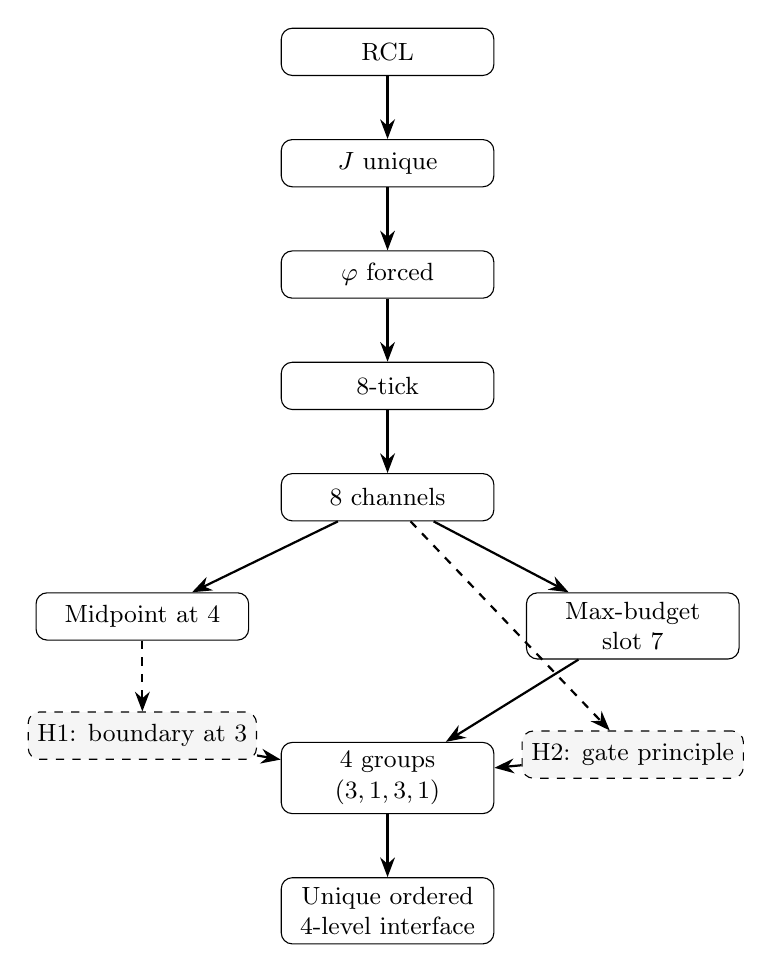
\begin{tikzpicture}[
  node distance=0.8cm and 1.8cm,
  box/.style={draw, rounded corners, minimum width=2.7cm,
    minimum height=0.6cm, font=\small, align=center},
  bridge/.style={box, dashed, fill=gray!8},
  arrow/.style={-{Stealth[length=2.5mm]}, thick},
  barrow/.style={arrow, dashed}
]

\node[box] (RCL) {RCL};
\node[box, below=of RCL] (J) {$\Jcost$ unique};
\node[box, below=of J] (phi) {$\phig$ forced};
\node[box, below=of phi] (tick) {8-tick};
\node[box, below=of tick] (slots) {8 channels};
\node[box, below left=0.9cm and 0.4cm of slots] (mid)
  {Midpoint at 4};
\node[box, below right=0.9cm and 0.4cm of slots] (maxb)
  {Max-budget\\slot 7};
\node[bridge, below=0.9cm of mid] (H1)
  {H1: boundary at 3};
\node[bridge, below=0.9cm of maxb] (H2)
  {H2: gate principle};
\node[box, below=2.8cm of slots] (four)
  {4 groups\\$(3,1,3,1)$};
\node[box, below=of four] (uniq)
  {Unique ordered\\4-level interface};

\draw[arrow] (RCL) -- (J);
\draw[arrow] (J) -- (phi);
\draw[arrow] (phi) -- (tick);
\draw[arrow] (tick) -- (slots);
\draw[arrow] (slots) -- (mid);
\draw[arrow] (slots) -- (maxb);
\draw[barrow] (mid) -- (H1);
\draw[barrow] (slots) -- (H2);
\draw[arrow] (H1) -- (four);
\draw[arrow] (H2) -- (four);
\draw[arrow] (maxb) -- (four);
\draw[arrow] (four) -- (uniq);

\end{tikzpicture}
\end{center}

\noindent Solid boxes: forced from the RS core. Dashed boxes: bridge
hypotheses.

\end{document}
